\subsection{Saliency Maps}
We trained a simple classifier to distinguish between dogs and wolves, using a \cite{ResNet} backbone network, on top of which we put a $2048 \to 1$ linear layer followed by a sigmoid. For this, we used the \cite{dogvwolf} dataset on Kaggle. \\ Let us take a look at an image and its corresponding saliency.
\begin{figure}[H]
    \centering
    \subfigure[]{
    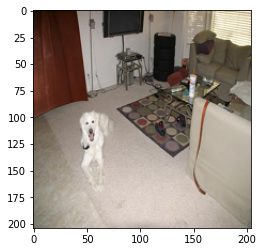
\includegraphics[width=.4\columnwidth]{2im.png}}
    \qquad
    \subfigure[]{
    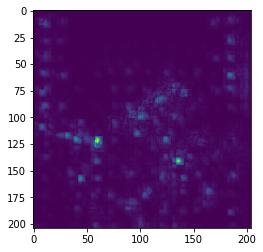
\includegraphics[width=.4\columnwidth]{2.png}}
    \caption[Short text]{Image and its Saliency Map}
\end{figure}
Through the previous result, we suspect a dependence on the background. Now, we look at an image from the test set which was classified as a wolf.
\begin{figure}[H]
    \centering
    \subfigure[]{
    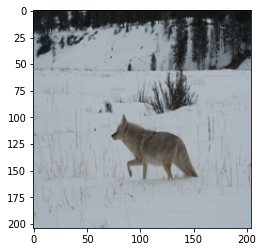
\includegraphics[width=.4\columnwidth]{3im.png}}
    \qquad
    \subfigure[]{
    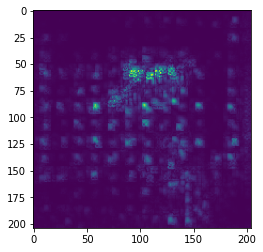
\includegraphics[width=.4\columnwidth]{3.png}}
    \caption[Short text]{Wolf  and its Saliency Map}
\end{figure}
We deliberately found an image of a dog with a white background, and fed it to the model to observe the following.
\begin{figure}[H]
    \centering
    \subfigure[]{
    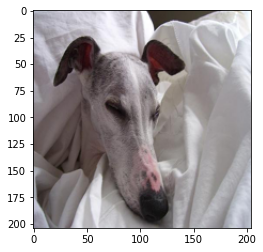
\includegraphics[width=.4\columnwidth]{4im.png}}
    \qquad
    \subfigure[]{
    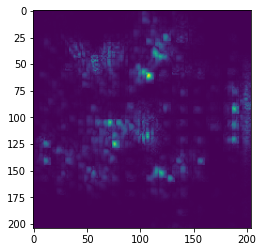
\includegraphics[width=.4\columnwidth]{4.png}}
    \caption[Short text]{A dog classified as a wolf}
\end{figure}
Thus, this technique enables us to comment on why certain classifications and particularly, some misclassifications are made.